\chapter{The GaitWatch Device}
\label{ch:gaitwatch}

\section{General description}
\indent GaitWatch is an Inertial Measurement Unit (IMU) designed for gait monitoring purposes. It was developed by Prof. Dr. Med. Kai B\"otzel at the Department of Neu\-ro\-lo\-gy of Ludwig-Maximilians University in Munich in conjunction with Dr. Alberto Olivares Vicente from the Department of Signal Theory, Telematics and Communications of the University of Granada. \\
GaitWatch is thought to be used in applications in which it is necessary to monitor the motion of patients. \\
\indent The system is composed of a box which contains the central processing unit and a set of measuring units which are wired to it. The measuring units are thought to be placed in the patients' thighs, shanks, arms and trunk. Figure XXXX shows the appearance of the complete GaitWatch device. 

\section{Hardware description}
\indent As it was aforementioned, GaitWatch has a box containing the central processing unit as well as a set of embedded magnetic and inertial sensors. The microcontroller acting as the central processing unit is in charge of gathering the data from the external measurement units and writing it to the memory card together with the data from the embedded box sensors. \\

\indent There are two different kinds of external units. The first one (type A IMU) is placed on both thighs and shanks. The second unit (type B IMU) is placed on both arms. Figure \ref{fig:GWdiagram} shows a diagram of the box (which contains the CPU and the type C IMU) together with the external units. 

\begin{figure}[H]
\centering
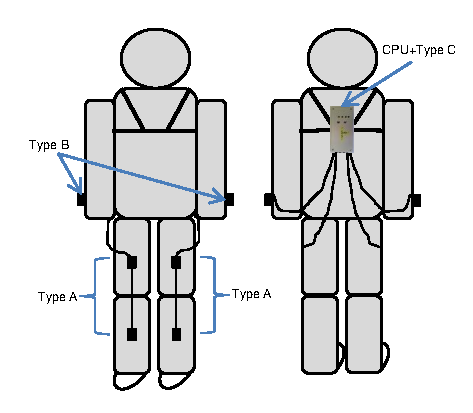
\includegraphics[width=0.8\textwidth]{figures/GWdiagram}
\caption{General diagram of the GaitWatch being worn by a subject.}
\label{fig:GWdiagram}
\end{figure}

\indent The three different kinds of IMUs have the following components:

\begin{itemize}
	\item Type A (thighs and shanks): 
	\begin{itemize}
		\item IMU 5 \cite{imu5} from Sparkfun. IMU 5 contains an IDG500 \cite{idg500} biaxial gyroscope (from which only Y axis is actually used) with a measurement range of $\pm500deg/s$ and a $\pm3g$ triaxial accelerometer, ADXL335 \cite{adxl335}.
	\end{itemize}
	\item Type B (arms):
	\begin{itemize}
		\item IDG500 \cite{idg500} biaxial $\pm500deg/s$ gyroscope.
	\end{itemize}
	\item Type C (trunk box):
	\begin{itemize}
		\item ADXL345 \cite{adxl345} triaxial accelerometer with programmable range ($\pm16g/\pm8g/\pm4g/\pm2g$).
		\item IMU3000 \cite{imu3000}triaxial gyroscope with programmable range ($\pm250/\pm500/\pm1000/\pm3000 (deg/s)$).
		\item Micromag3 \cite{micromag3} triaxial magnetometer ($\pm11Gauss$).
	\end{itemize}
\end{itemize}

In addition, the trunk box contains an AL-XAVRB \cite{avratx} board containing an AVR ATxmega processor which contains the necessary embedded firmware to gather the data from all the measurement units and store it in a microSD card.

Figure XXX shows the schematics of the complete GaitWatch device.

